
\phantomsection
\pagestyle{plain}

\begingroup

\let\clearpage\relax
\let\cleardoublepage\relax
\let\cleardoublepage\relax


\interlude{Mapping Animal Movement in \textit{R}}\label{box:mapping}
\noindent \textbf{Pratik R. Gupte}

\medskip

\setlist[description]{font=\scshape\bfseries\space}
\footnotesize
\begin{description}
	\item[Mapping as Exploratory Data Analysis] Mapping animal movements is a key component of exploratory data analysis. 
	It is important to `join the dots' of animal positions. Large tracking datasets can contain errors that are only evident to researchers when they look at an approximation of the animal's path and ask, ``Does the animal move this way?''
	This map shows `jumps': long, linear segments between points, indicating missing data for some periods. 
	
	Mapping can also reveal interesting behaviours that can only be observed after significant effort in the field.
	The `looping' behaviour of \emph{AM253} to water sources is the focus of this map. 
	Seeing this looping behaviour allowed us to focus our study on elephant movements between visits to water sources.
	
	\item[Mapping as Art] Growing up in early 2000s India, I read hard copies of National Geographic Magazine, which has long had fantastic graphics. \emph{Where the Animals Go}\footfullcite{cheshire2017} was a source of inspiration as well. I built up the image in layers, used colours that don't clash, and highlighted the phenomenon of interest. These approaches chime with the `grammar of graphics' approach of \textit{ggplot}, which I used to make this map.
	
	\item[Mapping in R] R's great advantage over other languages is visualisaton, specifically the popular \emph{ggplot} package. \textit{ggplot}'s emergence as a mainstay of spatial visualisation is due to its \textit{geom\_sf} function, which can handle sf spatial objects.

	One of \emph{ggplot}'s advantages is its many extensions. Here, I used the \emph{ggspatial} and \emph{ggtext} extension packages to add the scale bars and north arrow, and to add the text box, respectively.
		
	Plotting rasters is not straightforward in \emph{ggplot}. There are two main options: the stars package and its associated \textit{geom\_stars}, or converting a raster dataset into a dataframe with regular coordinate intervals and using \textit{geom\_tile}.
		
	Here, I chose the second approach because I'm an infrequent stars user; since making the map I've tried \textit{geom\_stars} which works just as well, and is very convenient.

	\item[Reproducibility in R] I adopted a relatively relaxed understanding of reproducibility: given the data, the code would be reproducible if it could produce the map I had entered for this contest. To do this, I set up a continuous integration pipeline using Github Actions (GHA).

	Using the \textit{usethis} package, I created a `DESCRIPTION' file, which is usually reserved for packages. This file tricks GHA into reading its contents, especially the dependencies, i.e., the R packages required by the project.

	GHA automatically reads the dependencies and installs them, as well as the programs required by those dependencies. For instance, GDAL (the Geospatial Data Abstraction Library) is key to nearly all spatial analyses, and is installed as a requirement of the \textit{rgdal} package, which is itself key to \textit{sf} and \textit{raster}.

	I used the R package \textit{renv} to make sure that the packages (and the package versions) I used are available to the pipeline. \textit{renv} creates a lockfile, a registry of packages the current project uses, from which those packages can be installed.
	Finally, to check whether the entire pipeline works, I used \textit{bookdown} to sequentially execute the series of Rmarkdown files. An obvious alternative is \textit{rmarkdown}.

	GHA runs this pipeline and reports whether the code ran successfully, and if not, where it failed (you can see these reports here). GHA runs the pipeline on Linux, and Windows containers (Mac OS-x is also supported). This means that though I use Linux, I'm pretty sure that this code works for Windows users.

	\item[The Limits of Reproducibility] Reproducibility inevitably breaks down at certain scales in an ecological study. For instance, it would be impossible to reproduce the primary data collection of the study, such as which elephants were captured and fitted with transmitters. These data are taken on faith from the original researchers, highlighting the role of trust in the scientific community.

	In ten years, code in R or another language may no longer be reproducible due to software and hardware changes, as many researchers found in the 10-year reproducibility challenge. Finally, entire services might become unavailable; for example, the raster processing using Google Earth Engine is dependent on Google maintaining this service.

	Researchers then, should be pragmatic about reproducibility. Who is it for — the researchers themselves, the reviewers of their manuscript, their students, their funders?
	To whom this effort is owed, and by whom, and how the additional work required can be prevented from becoming a gatekeeping mechanism \footfullcite{finley2017}\textsuperscript{;}\footfullcite{murphy2020}, are are issues that the ecology and evolution community will have to address.
\end{description}

% { \begin{center} \barfont{-.-} \end{center} }

\subsection*{About This Map}

This map and text is adapted from a submission to the \textit{Methods in Ecology and Evolution} blog, after my entry won the BES' Mapping Animal Movements Contest (2020 -- 2021), in the reproducible ``R Map'' category. The map shows the movement of 14 female savanna elephants \textit{Loxodonta africana} tagged in Kruger National Park, South Africa, with a focus on the elephant \emph{AM253}.
The study that inspired this map was published as \citet{thaker2019} \citetitle{thaker2019}.

I coloured the temperature raster using the \textit{scico} package's `VikO' palette. I tried out a number of palettes from \textit{scico}, pals (providing the Kovesi palettes), \textit{RColorBrewer}, and \textit{colorspace} packages. I chose a diverging palette to show heterogeneity in the thermal landscape, but this approach is not to be recommended for material that will be printed in grayscale.

Map text is set in two related typefaces designed by the Dutch type foundry \emph{Bold Monday} for IBM: \emph{Plex Serif} --- for text on the map --- and \emph{Plex Sans} --- for text in the box.
While aiming to be text typefaces, I think both perform much better as `display' faces; Plex Serif especially so.

{ \begin{center} \barfont{-.-} \end{center} }

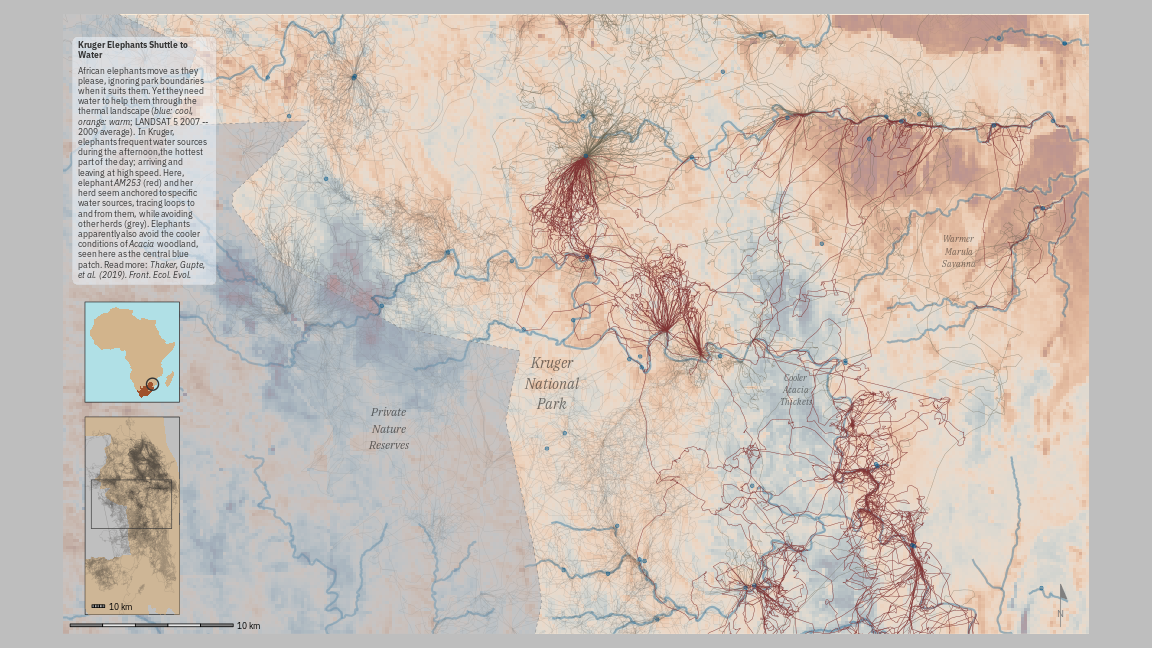
\includepdf{figures/boxes/elemove.pdf}

\endgroup

\afterpage{\nopagecolor}
\pagestyle{scrheadings}
